%!TEX root = ../main.tex

\section{Geschichtliche Entwicklung}
    \begin{frame}<beamer>{geschichtlicher Hintergrund}
      \begin{figure}
        \begin{subfigure}[b]{0.5\textwidth}
          \begin{itemize}
            \item
              Telekommunikation bedurfte früher die Verbindung von zwei Anschlüssen
            \item
              erste hälfte des 20. Jahrhunderts Einführung von Vermittlungsstellen
            \item
              Verbindungszähler addieren nur die Gebühren
            \item
              Einführung von Fangschaltungen
            \item 
             ab ca. 1980 Einführung von digitaler Vermittlungsgeräte
            \item
              Aufzeichnung von Rufnummern automatisch
            \item
              Erlaubte Speicherung nur zur Abrechnung
            % Kommentare
            % - Pruefung 2005 war ob und welche Dinge erlassen werden sollten
            % - Vorschlag von 2004 beinhaltete 36 Monate Speicherung, auch fuer Filesharing..
            % - Initiiert von Frankreich, Irland, Schweden und UK
            % - Ministerrat sieht es als seine Zustaendigkeit 'Dritte Saeule der EU'
            % - Parlament sieht es als seine 'Erste Saeule der EU'
            % - Kommision sagt beide
          \end{itemize}
        \end{subfigure}
        \begin{subfigure}[b]{0.3\textwidth}
          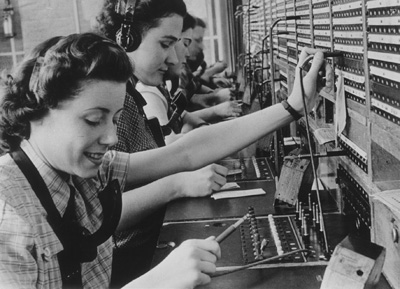
\includegraphics[scale=1]{sections/img/vermittlungsstellen.jpg}
          \caption{Vermittlungsstelle}
          \label{fig:vermittlungsstelle}
        \end{subfigure}
      \end{figure}
    \end{frame}

